% Created 2021-09-13 Mon 22:45
% Intended LaTeX compiler: pdflatex
\documentclass[11pt]{article}
\usepackage[utf8]{inputenc}
\usepackage[T1]{fontenc}
\usepackage{graphicx}
\usepackage{grffile}
\usepackage{longtable}
\usepackage{wrapfig}
\usepackage{rotating}
\usepackage[normalem]{ulem}
\usepackage{amsmath}
\usepackage{textcomp}
\usepackage{amssymb}
\usepackage{capt-of}
\usepackage{hyperref}
\author{Jay Kruer}
\date{\today}
\title{9/14: Up to Speed on Sterling \& Spitters}
\hypersetup{
 pdfauthor={Jay Kruer},
 pdftitle={9/14: Up to Speed on Sterling \& Spitters},
 pdfkeywords={},
 pdfsubject={},
 pdfcreator={Emacs 27.2 (Org mode 9.5)}, 
 pdflang={English}}
\begin{document}

\maketitle
\tableofcontents

\section{Reminders of some notions from my first chapter}
\label{sec:org36fc68a}
Review the category of contexts and substitutions, I can do this live.
\section{The Yoneda embedding and normalization by evaluation}
\label{sec:org453ef65}
\subsection{Normalization? Evaluation?}
\label{sec:org58d62f4}
Normalization by evaluation is a technique used to demonstrate normalization--
the property that all terms have a normal form--for some lambda calculus.
Andreas Abel renders the technique very clearly\footnote{\url{https://www.cse.chalmers.se/\~abela/talkEAFIT2017.pdf}}: Normalization is the
process of bringing an open term (with unknowns) to a special kind of fixed
point. A similar notion is evaluation, the process of bringing a \emph{closure},
namely an open term paired with a substitution closing it, to a canonical form
comprised entirely of constructors.

\textbf{Normalization by evaluation} borrows an exist evaluator for some sufficiently
expressive host language and uses it to normalize an open expression in the
guest language we're interested in. The basic plot outline is this, each step
paired with the relevant code from an instance\footnote{\url{https://en.wikipedia.org/wiki/Normalisation\_by\_evaluation}} of normalization with the host
being Standard ML and the guest being the simply typed lambda calculus:
\begin{enumerate}
\item Create in the host language an internal representation of the guest language syntax and type structure:
\begin{verbatim}
    datatype ty = Basic of string
                | Arrow of ty * ty
                | Prod of ty * ty

    datatype tm = var of string
                | lam of string * tm | app of tm * tm
                | pair of tm * tm | fst of tm | snd of tm
\end{verbatim}
\item Building a semantic model (a la actions) of the guest language in terms of host language constructs:

\begin{verbatim}
   datatype sem = LAM of (sem -> sem)
                | PAIR of sem * sem
                | SYN of tm
\end{verbatim}

   Here, our model expresses lambda expressions in STLC as \emph{actual ML
functions} and pairs as \emph{actual ML pairs}. We also allow for embedding syntax
terms of our base type, which have no further structure, into the semantics.

\item Defining a mutually recursive pair of type-indexed operation families called
reification and reflection, detailed in the next section, whose composition
acts as a normalization function.
\item Compose reification with reflection to get a normalization function for terms
in the guest language.
\end{enumerate}

\subsection{Reflection, reification}
\label{sec:org4f70c8b}
\begin{center}
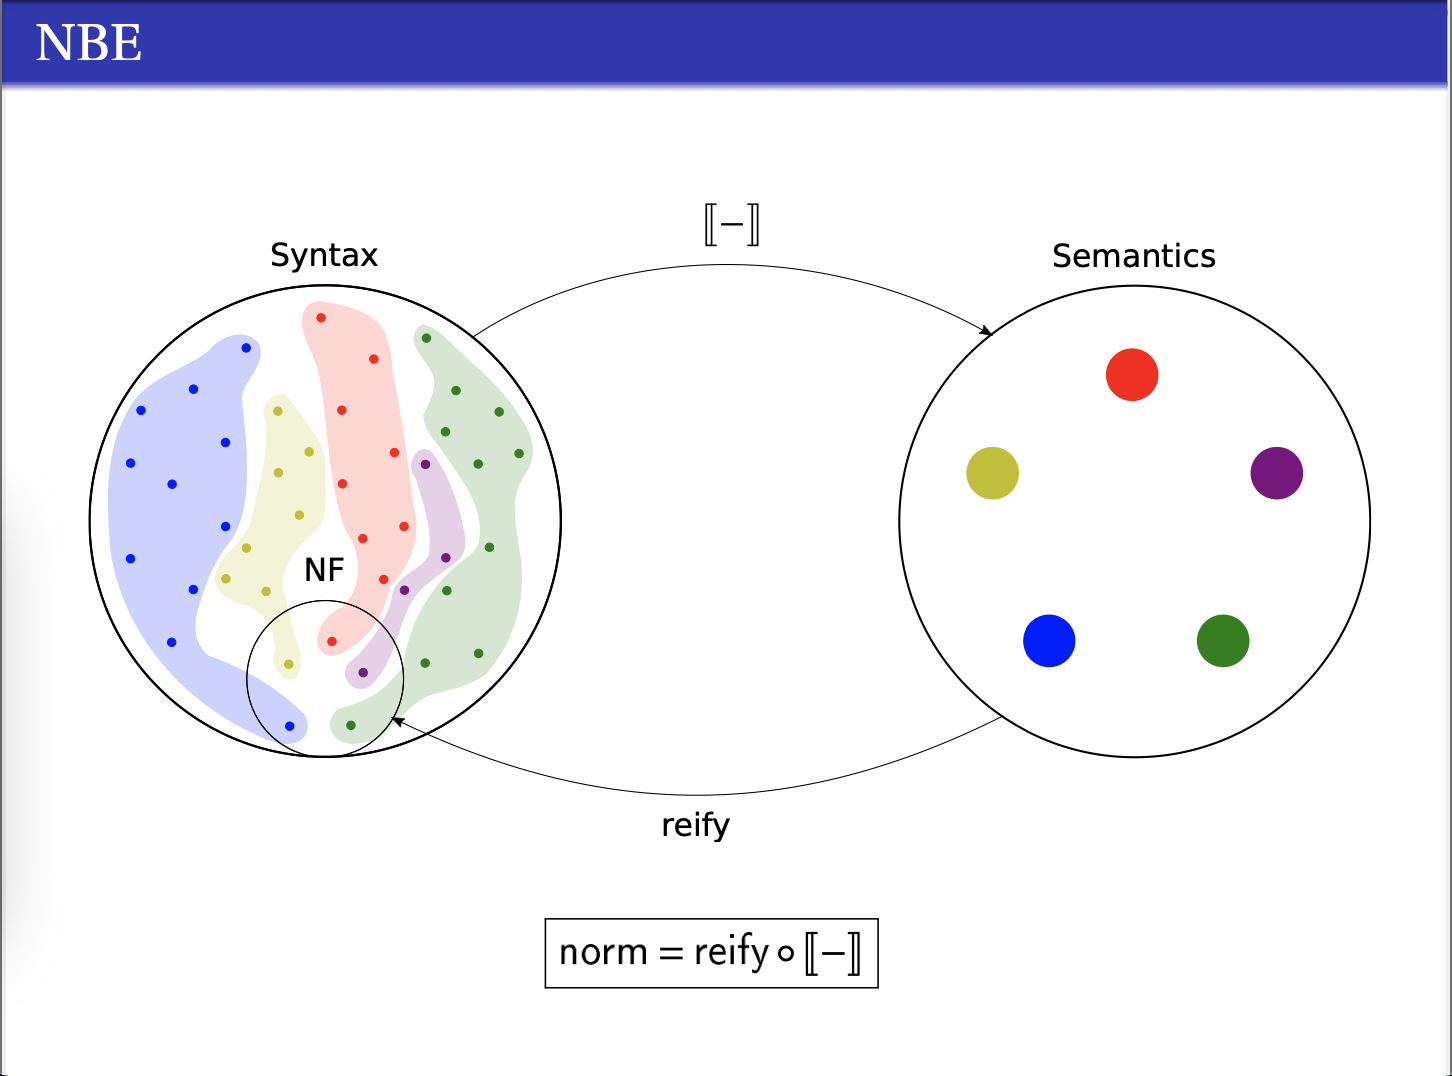
\includegraphics[width=.9\linewidth]{nbe.png}
\end{center}
Reflection is the operation which takes a syntactic lambda term, namely
something in \texttt{tm}, and produces the corresponding semantic representation in
\texttt{sem}. The instance from Wikipedia features the following reflection operation
defined mutually with reification:
\begin{verbatim}
 (* reflect : ty -> tm -> sem *)
 fun reflect (Arrow (a, b)) t =
       LAM (fn S => reflect b (app t (reify a S)))
   | reflect (Prod (a, b)) t =
       PAIR (reflect a (fst t)) (reflect b (snd t))
   | reflect (Basic _) t =
       SYN t

(* reify : ty -> sem -> tm *)
 and reify (Arrow (a, b)) (LAM S) =
       let x = fresh_var () in
         lam (x, reify b (S (reflect a (var x))))
       end
   | reify (Prod (a, b)) (PAIR S T) =
       pair (reify a S, reify b T)
   | reify (Basic _) (SYN t) = t
\end{verbatim}

I'll start my explanation of this with reification, because it will come first
in the normalization function we're building. In its first case, we want to
reflect a syntactic function (something of arrow type) into our semantics. To do
so, we create a new ML function (with a lambda expression) which reflects into
the semantics the result of applying the syntactic function to the reification
of its parameter. This resembles the usual eta-expansion for terms of function
type, in which we take \(f: A \rightarrow B\) to the term \(\lambda a.\, f a\). The pair case has a similarly eta-expansive flavor. The case for the base
type just embeds the term into the semantics.

Reification is just like reflection but with the parity of
reflection/reification calls flipped everywhere. As before, for function types
we perform something like eta-expansion; only here we can't rely on the
meta-language to handle variable freshness issues and we have to allocate
hitherto-unbound variables ourselves. Pairs are similar, without the variable
complication. The case of the base type amounts to undoing the embedding
performed by reflect.

One can show that the composition \texttt{fun t. reify (reflect (t))} is a normalization
function for the simply typed lambda calculus.

\subsection{Back to SterSpit}
\label{sec:orgcf3dc70}
The first big claim in SterSpit is that a special version of the Yoneda
embedding (with more intensional flavor) defines a reflection operation from the
syntactic category into its category of presheaves. SterSpit promise a
corresponding reification operation to complete the normalization by evaluation
story, but delay its introduction until a few sections past what I've managed to
understand so far. For now, we have a problem.

\section{A pickle: too much quotienting}
\label{sec:org291590c}
The definition of the syntactic category (category of contexts and
substitutions) given in the chapter I wrote a few weeks ago has for its
equations governing equality of morphisms those given by the ``substitution
lemma.'' It turns out that this identifies far too many terms for our uses. In
particular, terms which are related by the various beta rules are identified,
meaning that a normal form (a term for which no further beta reduction can be
performed) is identified with its (manifestly not normal) beta-predecessor. The
upshot is that we can't isolate the normal forms as a class of terms, which
totally bungles our whole project of investigating which terms (all of them) of
the simply typed lambda calculus have normal forms. To spell it out: the
normalization by evaluation function SterSpit propose is actually equal to the
identity on the syntactic category. The whole point of using the gluing
construction is to get us out of this situation by introducing more
computational information that allows us to distinguish terms from their
beta-ancestors and beta-posteriors.

\section{Unpickling ourselves: the category of renamings}
\label{sec:orgf07bb7c}
As an alternative to the misbehaving category of contexts and substitutions, we
will work with the catetory of renamings. In simple terms, this category has as
its objects all contexts over our types and whose morphisms are type-preserving
changes of variable from one context to another. Unfortunately as I found while
typing this up, the simple rendition is somewhat ill-specified. Fiore (2002)
defines this category as the opposite of the comma category \(\mathfrak{i}
\downarrow \mathfrak{T}\) where \(\mathfrak{i}\) is the functor embedding the
category \(\mathbb{F}\) of finite sets of variables (drawn from the supply of
our algebraic theory) into \(\mathfrak{Set}\) and \(\mathfrak{T}\) is the
constant functor for our set of types \(\mathfrak{T}\). Concretely, its
objects are maps \(\Gamma : V \rightarrow \mathfrak{T}\), i.e., exactly
contexts assigning types to finitely many variables. The morphisms \(\Gamma'
\rightarrow \Gamma\) (of the opposite we'll be working with) are functions \(\rho : \text{dom}(\Gamma) \rightarrow \text{dom}(\Gamma')\) such that \(\Gamma
= \Gamma' \circ \rho\), i.e., the morphisms are type-preserving changes of
variables. The reason we work with the opposite of this category is so that the
action of the category of the renamings acts contravariantly on the clones of
the syntactic category it embeds in; i.e., we want the arrows to line up with
the syntactic category.

\section{The relative hom functor}
\label{sec:org29ac52e}
Sterling \& Spitters follow Fiore in defining the ``relative hom functor'', which
they suggestively call \(\mathfrak{Tm} : \text{Cl}_{\Sigma} \rightarrow
{\text{Ren}_\Sigma}^{\mathfrak{Set}}\). The suggestion hinted at by the name,
that this functor defines a presheaf of open terms, turns out to be a small lie.
Let's look at what it actually does. \(\mathfrak{Tm}\) is defined by adjusting
the hom functor (i.e, the Yoneda embedding) by precomposition with the inclusion
of the category of renamings into the category of (contexts and) substitutions.
In particular, SterSpit define \(\mathfrak{Tm}(\Delta) = \text{Cl}_{\Sigma}
[i(-), \Delta]\). In plain terms, \(\mathfrak{Tm}(\Delta)\) takes a context in
the category of renamings to the \emph{substitutions on terms} \textbf{out of} \(\Delta\)
(recalling that the action of the category of contexts on its clones is
contravariant). This can be construed as a presheaf of open terms. For any type
\(\tau\) and any context \(\Gamma\), the morphisms in this set are (in their
totality):
\begin{enumerate}
\item Single substitutions \([t / x]\) where \(\Gamma \vdash t : \tau\). (Note
that this includes renamings); and,
\item Context weakenings \(\hat{y}\)
\end{enumerate}

Ignoring the weakenings, we see that we have a presheaf of open terms closed by
\(\Gamma\).

The suggestion does break down when generalizing the target context from a
single \(\tau\). For contexts \(\Delta\) and \(\Gamma\), we have
\(\mathfrak{Tm}(\Delta)(\Gamma) = \text{Cl}_{\Sigma} [i(\Gamma), \Delta]\), the
context \(\Gamma\) just falls through the inclusion and we get the
substitutions \(\gamma^{*} : \Delta \vdash \tau \rightarrow \Gamma \vdash \tau\) for arbitrary \(\tau\). Now here comes the (small) lie: the morphisms in
the syntactic category aren't just single substitutions, but also (as before)
single omissions \(\hat{x}\) and all the compositions of these two classes of
maps.
\end{document}
